\documentclass{article}
\usepackage[utf8]{inputenc}
\usepackage{graphicx}
\setlength{\headsep}{40pt}
\usepackage{geometry}
\geometry{a4paper}
\geometry{left=2.5cm, right=2.5cm, top=2.55cm, bottom=2cm}
\bibliographystyle{unsrt}
\usepackage{fancyhdr}
\pagestyle{fancy} 
\fancyhf{} 
\fancyhead[L]{
\includegraphics[height=1.15cm]{label.png}}
\renewcommand{\headrulewidth}{1pt}
\cfoot{\thepage} 
\usepackage{amsmath}
\usepackage{hyperref}
\usepackage{cleveref}
\usepackage{amsthm}
\usepackage{lipsum}
%\usepackage{biblatex}
\usepackage{natbib}
\usepackage{multicol}
\usepackage{amsfonts} 
\usepackage{bbm}
\usepackage{subfiles}
\usepackage{xcolor}
\usepackage{indentfirst}
\usepackage{listings}
\definecolor{codegreen}{rgb}{0,0.6,0}
\definecolor{codegray}{rgb}{0.5,0.5,0.5}
\definecolor{codepurple}{rgb}{0.58,0,0.82}
\definecolor{backcolour}{rgb}{0.95,0.95,0.92}
\lstdefinestyle{mystyle}{
    backgroundcolor=\color{backcolour},   
    commentstyle=\color{codegreen},
    keywordstyle=\color{magenta},
    numberstyle=\tiny\color{codegray},
    stringstyle=\color{codepurple},
    basicstyle=\ttfamily\footnotesize,
    breakatwhitespace=false,         
    breaklines=true,                 
    captionpos=b,                    
    keepspaces=true,                 
    numbers=left,                    
    numbersep=5pt,                  
    showspaces=false,                
    showstringspaces=false,
    showtabs=false,                  
    tabsize=2
}

\newcommand{\MGcomment}[1]{\textcolor{blue}{#1}}

\lstset{style=mystyle}
\title{PhD Thesis Research Proposal \\ Department of Informatics, University of Oslo}
\author{Liang Cheng}
\date{May 2024}
\usepackage{amsmath}
\numberwithin{equation}{section}

\begin{document}

\maketitle

\MGcomment{Some general comments here :-)}

\MGcomment{Some of the references use an ‘ampersand’ character \& that has to be escaped with a backslash.}

\MGcomment{The right way of referring to a figure or similar is Fig.~\ref{fig:overview}, look at the TeX code.  The tilde prevents a line break between the number and the abbreviation as well as making sure that the spacing is correct.}

\MGcomment{Don’t use straight "double" or 'single' quotes.  There is a difference between left and right quotes and the easiest way is to use the correct unicode characters like ‘this’ or “this”}

\MGcomment{There’s a space between a word and the cite command like this \cite{Forti20}. To avoid a line break, do this~\cite{Forti20} or this\ \cite{Forti20}}.

\MGcomment{Also, please don’t change the page geometry.  You may awant to add options 11pt or 12pt to the document class though.}

\MGcomment{The UiO seal in the heading: either use this in high quality vector graphic (\url{https://www.uio.no/om/designmanual/profilelementer/logo/}) or (much easier and just as good) don’t use it at all.}

\section{Project title}
Automated and Intelligent Data Flow Management for E-Waste 

Main Supervisor: Amir Taherkordi 

Co-Supervisor: Martin Giese

\section{Main objective and summary of the project}
\begin{figure}[h]
\centering
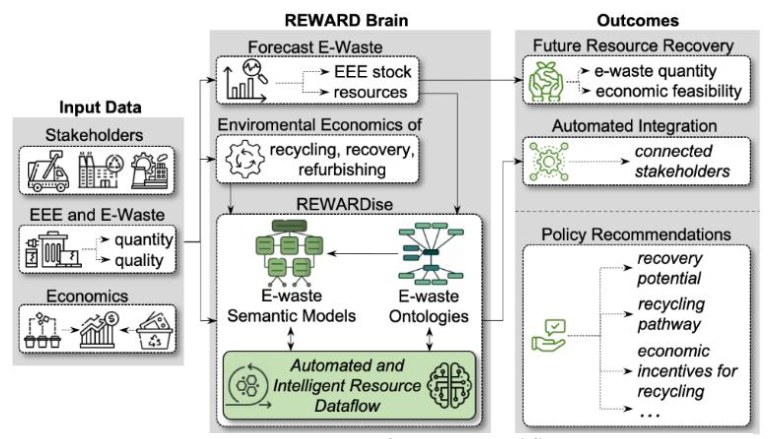
\includegraphics[height=6cm,width=10cm]{overview.png}
\caption{Overview of REWARD workflow} \label{fig:overview}
\end{figure}
With the continuous updating and iteration of electronic products, electronic waste (e-waste) is being produced at an unprecedented speed. Although these outdated or broken electronic products are considered to be waste, the materials and components they contain, and even the devices themselves, have considerable recycling value and have the opportunity to be reused in certain ways. Therefore, on this basis and with the promotion of relevant policies in the EU to encourage recycling of critical raw materials (CRMs), increasingly more \MGcomment{more and more, or an increasing number} companies have entered the recycling industry, but most of the recycling work is inefficient so far. There are many reasons behind this, such as insufficient tools to better integrate data from different sources, \MGcomment{this is a bit abrupt here.  Why is data integration the first challenge for e-waste handling?  I think it would make more sense to first explain the challenge, and then get to why data and data integration are important} and the lack of comprehensive recycling strategies and resource planning.

In this context, \MGcomment{the} REWARD project proposes a comprehensive system, which integrates many tasks that were not included in the previous e-waste recycling process, including data collection and integration, classification and matching in the recycling, and detailed recommendations for resource planning and policy development. The overview of REWARD workflow is shown in Fig \ref{fig:overview}. This PhD project is one of the key parts in \MGcomment{the} REWARD project that is mainly associated with e-waste data operating. Under this project, a new intelligent model with ontologies is required to harmonize the e-waste data across various data providers, including formats, representations, etc. \MGcomment{again, it would be better to first explain what needs to be done, before concluding that we need ‘intelligent models,’ ontologies, etc.} On the basis of a unified ontological system, there will be a clearer overview of how different products, components and materials in e-waste are related to each other, which enables us to construct an automated data flow system to better manage the data from different sources. In addition, further complicated computation can be performed in an efficient way with the use of cutting-edge semantic modeling and machine learning techniques to better match the shared e-waste data with actors’ requirements that eventually leads to the optimal resource planning. 
The primary objective of this PhD project is to conduct basic theoretical and experimental research to design and develop an automated and intelligent data flow management system \MGcomment{what is a ‘data flow management system’?} for e-waste to improve the overall performance in the recycling process. A significant difference from previous related domain models \MGcomment{where does the domain model come from? You just wrote that you want to build a data flow management system?} is that it involves ontology technology, which makes the integration of heterogeneous data convenient. In general, it provides a solid foundation for improving data quality, and facilitating data discovery and querying. Ontology and semantic modeling have been shown in many other applications to be used in conjunction with machine learning techniques to improve model performance, and these cases provide a way forward for this research.

\section{Project background and scientific basis}
\MGcomment{There is too much detail here that is not important to understand your project. Also, if parts of the text are copied from the proposal text, they should be attributed.}

Only 2.4\% of the 235 million tonnes of materials consumed in Norway each year are recovered through recycling. The remaining share (97.6\%) may be lost in the use of stockpiles (consumer durables) and/or in waste disposal processes, and e-waste is one of  the fastest growing waste streams among them. E-waste is mainly described as waste generated from all parts and articles of electrical and electronic equipment (EEE) that have been discarded and are not intended for reuse. An important characteristic of electronic devices is their short lifespan, which makes all of them destined to become e-waste within a certain period of time, although the time may vary depending on the type of product, from a few months to a few years. In addition, manufacturers produce next-generation information and communication technology (ICT) and EEE at a frenetic pace, constantly introducing them into the increasingly saturated market as "cutting-edge" must-have technology for customers. This leads to increasing requirements and expectations from customers on electronic products, and directly accelerates the obsolescence of old products that need to be properly disposed of or recycled. As a result, the growth of e-waste\cite{Forti20} is on a fast track and the volume of e-waste is increasing at a more rapid rate each year.

As the volume of e-waste surges, the improper handling and disposal \cite{Shaha22}of these electronic products pose significant environmental and health risks. E-waste contains a wide variety of materials including metals, glass, plastics, and hazardous substances such as lead, mercury, and brominated flame retardants, which means that they can not be recycled in their entirety like other waste, but need to be broken down into individual component or even material first, depending on specific recycling needs. Classifying the different components or materials, and matching them to the specific needs of the recycling actors can be an expensive and time-consuming process. Besides, there is a lack of a comprehensive standardized e-waste recycling policy\cite{why22} across different countries, areas and even companies, which exacerbates the difficulty of recycling e-waste. Although some companies, such as Apple, offer recycling options to their customers, there is no agreed and approved recycling policy that sets out the safest and most efficient way to recycle and manage all types of e-waste. 

As there is currently no specific e-waste recycling policy to guide governments, companies and individuals in the e-waste recycling process\cite{ramz08}, this has encouraged the prevalence of informal recycling practices. In many regions, e-waste is managed through these informal channels, which often involve hazardous and unsafe e-waste disposal methods. Furthermore, the absence of tracking e-waste data flows in informal recycling makes the process less transparent, which may lead to underutilization of recycled materials or reduced recycling efficiency. In recent years, green transition related policies have arisen in Europe that advocate the utilization of renewable technologies and digital infrastructures, which leads to an increasing demand for CRMs. These policies have put forward higher requirements for the classification and recycling of e-waste, including more detailed classification requirements and a more efficient recycling process. All these together, making constructing an unified e-waste data management infrastructure essential,  in order to improve the efficiency of e-waste recycling and the utilization rate of e-waste after recycling, and minimize harm to the environment as well as to humans.

A number of challenges related to the data itself have persisted in the process of establishing a comprehensive e-waste data management system, including the complexity, heterogeneity and lackness of e-waste data. When it comes to the complexity of e-waste data\cite{ea22}, e-waste can be divided into multiple classes  in terms of hierarchy, which mainly includes product level, component level and material level. With cellphone as an example, at the product level, there will be a great number of cellphone brands in the recycling process, and even for the same brand, there will be various models of cellphone under process. At the component level, cellphone can be disassembled into a number of different parts, such as screen, sensors, battery and so on. All of these individual components have the opportunity to be reused and assembled into new products with other components from other products. As for material, it is the fundamental level that all the components are constructed from materials. For a cellphone, there will be a variety of materials, including metal, plastic, glass, etc. Although materials may come from different components and products, some actors in the recycling process may aim to recycle a specific material, which makes the recycling process more difficult and highlights the need for e-waste data management. Beyond that, another important aspect of e-waste data in complexity should be taken into account when managing the data flow, namely its dynamic nature. As mentioned before, the lifespan of most electronic devices is relatively short, so there could be an influx of e-waste in a short period of time. It indicates that the data management system should be robust enough to dynamically adopt new data and digest the new-coming knowledge and information.

Up to now, there are multiple companies engaging in the e-waste recycling business\cite{matt23} in Norway, and e-waste management practices vary significantly across regions for them. Each of these data providers has its own regulations in recording and managing the e-waste data, which results in the heterogeneity across the data format and description for the same e-waste. For example, some data providers would record the information of a recycled laptop such as weight and price into a table as structure data, while the others might use the text to summarize this information directly. Meanwhile, different terms sometimes can refer to the same e-waste, like laptop and notebook are both commonly used to represent the portable computers. As a result, various discrepancies between different data sources can cause inevitable confusion in the processing of e-waste data and increase the inconvenience of data flow maintenance.

The lack of e-waste data is also a potential issue that has to be taken into consideration in the construction of an efficient and comprehensive data flow management system. The problem is of two aspects, firstly the lack of data sources and secondly the lack of certain specific types of data. It is known to us that a significant number of companies do participate in the e-waste recycling industry, but it doesn't necessarily mean that all of them are willing to share their e-waste data, as some of them may consider doing so to be against their business interests. It requires an establishment of a trustworthy data management system to ensure an integration of data from various sources without causing commercial and ethical conflicts. In the situation that some companies are willing to share data, it is also possible that the majority of these data sources are focusing on some certain types of e-waste or that their business has not covered all e-waste for the time being, leading to a lack of data on certain types of e-waste. Without the support from a comprehensive database, it could be difficult to perform accurate matching operations to link the e-waste with actors’ recycling requirements.

In the field of information science, an ontology is a formal representation of knowledge within a particular domain that encompasses the concepts, entities, relationships, and attributes relevant to that domain\cite{sat20}. In the context of e-waste, various elements can be encoded to an ontology such as types of electronic devices, components that devices contain, materials used in their construction or even other relevant information like recycling processes and environmental impact factors\cite{rama15}. In addition, ontologies excel at representing the rich web of relationships that exist within the e-waste domain. For instance, they can not only capture hierarchical relationships between different types of electronic devices (e.g., smartphones, laptops, printers) and the components they contain (e.g., circuit boards, batteries, displays) but also encode semantic relationships such as "is-a" (e.g., a smartphone is a type of electronic device) and "has-a" (e.g., a laptop has a battery). The properties of the ontology is a good fit for the complexity of e-waste data, which is able to well illustrate both explicit and implicit relationship among different parts of e-waste. Besides, ontologies provide a unified framework that makes it possible to create a standardized model that facilitates data integration and interoperability between different systems and datasets\cite{dara16}.

Semantic modeling builds upon ontologies, encompasses various techniques and methodologies for leveraging ontologies to represent, structure, and analyze data in a way that captures its semantics\cite{band19}. Due to the complexity and diversity of information involved in the e-waste domain, semantic modeling is a valuable approach to organizing, integrating, and analyzing e-waste data. On the basis of ontology development, the ontology-based techniques can be applied on constructing semantic model, including ontology language and knowledge graph\cite{gon17}. The former can be used to create a formal representation of the e-waste domain, which involves defining classes, attributes, and relationships in an ontology that wraps the semantics of the e-waste data. The latter represents e-waste data in a graph-based format. Entities such as electronic devices, components, materials and recycling processes are represented as nodes in the graph, while the relationships between them are represented as edges. This graph structure allows for the seamless integration of heterogeneous e-waste data from different sources\cite{ange22}, thus allowing for efficient querying and analysis across different datasets. 

In addition to semantic representation building, this project lends itself to the use of other semantic modeling techniques, such as ontology alignment\cite{Shva13} and semantic embedding\cite{penn14}, which are significant for downstream tasks based on semantic representations. Ontology alignment is the process of harmonizing and integrating ontologies from different domains to ensure interoperability and consistency, and in the context of e-waste, it can refer to ontologies built from different sources. This involves identifying correspondences between entities, attributes and relationships in different ontologies and establishing mappings or alignments for seamless communication. As for semantic embedding, it refers to representing words, concepts, or entities in a continuous vector space, mapping semantically similar items to nearby points. This technique captures the underlying semantic structure of data by encoding semantic relationships and similarities into a low-dimensional vector representation. The embedding methods can vary to some extent in the field of e-waste depending on the semantic representation used.

Different machine learning and deep learning techniques can be applied to different stages of semantic modeling depending on the data and some other specific requirements. One common use of machine learning is applied on ontology construction, which aims to capture some preferred patterns or achieve automation. The authors in \cite{yan08} proposed an approach that incorporates periodical manual guidance into a supervised clustering algorithm when constructing ontology to capture personal preference in the data. The authors in \cite{al20} summarized the recent research in using deep learning to achieve automation for ontology construction from text. Further than ontology, machine learning techniques also can be used on constructing knowledge graph to avoid the complicated manual operation. The authors in \cite{zhao24} explored the the use of machine learning in different stage of knowledge graph construction and analyzed its impact. Ontology Alignment using machine learning was investigated in \cite{nezh11} to optimize the model performance. Most tools in semantic embedding such as Word2Vec\cite{miko13}, GloVe\cite{penn14}, and fastText\cite{boja16} based on deep learning that use co-occurrence statistics or neural network architectures. Downstream tasks based on semantic embedding, such as matching, classification, and prediction, are also common application areas for machine learning and deep learning, as the data to be processed at this stage are ordinary vectors, which are the same inputs as for most classical machine learning and deep learning tasks. 

Although most existing researches in the field of semantic modeling and machine learning like those mentioned above are not associated with e-waste, they brought novel ideas and insight about how can machine learning and semantic modeling cooperate with each other, and the collaboration between machine learning and semantic modeling can be further modified considering the unique features of e-waste data and specific requirements of REWARD project. 

\section{Research questions and scientific challenges}
This PhD project will address the following questions, which will begin with the aspect of e-waste data itself, and then progressively focus on the detailed functionality of the tool that processes these data to achieve our research goals. \\

\textbf{Research Question 1 (RQ1)}: How to define a unified semantic system to describe e-waste knowledge facing the continuous changing data?

When constructing a big data platform, the first thing to consider is the characteristics of the data, as one of the keys to make the platform efficient is to ensure that it fits well with the data. In the scenario of the e-waste recycling system, the data mainly comes from two sides, e-waste itself and actors, which are e-waste acceptors in the recycling process. From the perspective of e-waste, the complexity, heterogeneity, lackness and the dynamic nature discussed in the previous section are some of the most significant features that we have to take into account. In order to model a well-developed semantic system for e-waste, a large amount of e-waste knowledge is required, which includes not only the e-waste data from data provider but also domain knowledge from other research areas related to e-waste, such as structural information of e-waste, manufacturing process and recycling process. When these different sources and perhaps even different disciplines of knowledge come together, complexity and heterogeneity are magnified even further, and this is where a unified semantic system becomes particularly crucial. A unified semantic system would provide a common language or set of standards for describing e-waste knowledge to avoid confusion, making it easier to manage and analyze data from different sources and contexts.

In addition, unlike many other static data, the status of e-waste data is likely to be updated frequently because the recycling system is dynamic and policies and planning regarding recycling would also change over time, indicating there is always new data coming in and old data going out, which makes timely status updates significant for accomplishing the downstream tasks. Although this is not a demand for real-time updates, the situation of continuous changing data still poses higher requirements compared to general semantic modeling. Therefore semantic modeling incorporating dynamic mechanisms would be a promising solution to the problem.\\

%For one e-waste, it generally contains multiple components, and various materials could be included in one component. Different products in e-waste have a chance to share the same component or material information. Not to mention that there is much other information highly related with the recycling result that would be encoded in the e-waste data, such as manufacture, price and recycling procedures. This inherent complexity of e-waste data makes it difficult to be processed into a structured framework with a clear vision. In order to implement an efficient data management system, massive amounts of data are required, which suggests that integrating data from numerous different sources is necessary. However, one issue we need to counter when handling heterogeneous data is data interoperability. For various data providers, it is inevitable that they utilize different representations or formats for recording similar data, taking into account that each data provider has its own unique data recording system and may focus on different perspectives of e-waste data. A proper standard should be proposed to avoid confusion in understanding the difference across multiple data sets for data integration. In general, the lackness problem can appear in different forms for both e-waste and actors' sides. For the e-waste side, this issue normally comes in the lack of some specific kinds of data leading the the incomplete semantic model and causing troubles for the later downstream task such as matching. But this can be addressed as more and more data is adopted into the system. On the other hand, the lackness on the e-waste acceptor side is not easy to be solved since some of the data providers are only in charge of collecting e-waste but not assigning them to the acceptors, which causes the amount of information from the acceptors could be much less than that from e-waste side. Unlike many other static data, the status of e-waste data is likely to be updated frequently because the recycling system is dynamic, and there is always new data coming in and old data going out, which makes timely status updates significant for accomplishing the downstream tasks. Although this is not a demand for real-time updates, it still poses higher requirements compared to general semantic modeling. \\

\textbf{Research Question 2 (RQ2)}: How to connect actors and e-waste data under semantic modeling automatically in consideration of different levels (product, component, material) of recycling?

One of the primary goals for constructing this e-waste management system is to make the matching between e-waste data and acceptor faster and more accurate, which can in turn improve the efficiency of the overall recycling process.  The key points to explore here are automaticity and accuracy improvement. %The connection between e-waste and acceptors should be anonymous during the recycling. Although the e-waste recycling is aimed at protecting the environment, it is still a commercial activity and we will use some confidential information in model construction, so it is important to protect the security of the acceptor's information during the recycling process to prevent the leakage of information. 

Achieving automaticity is one significant step in improving recycling efficiency. Up to now, there are a number of existing e-waste management systems in place, but most of them require manual operation, which not only reduces productivity but also has the potential to introduce human error into the system to lower the accuracy of matching. As mentioned in RQ1, the dynamic nature of e-waste data would require a frequent updating of semantic model, so automated integration, processing and analysis of data is essential to ensure timeliness and efficiency. In addition, as the volume of e-waste increases over time, manual management will become increasingly impractical, and automation is key to ensure that the management process remains robust and reliable.

Although automaticity plays an important role in the matching, the essential part of this research question is to identify and establish the link between the e-waste and the possible acceptors. Due to its particular complexity, e-waste can be categorized into different levels (product, component and material). However, from the perspective of data itself, there are not only certain direct and indirect correlations between the different levels of e-waste data but also some partial overlap among them, which complicates this question to some extent. For example, one wasted phone can be regarded as a phone at the product level, it also has a camera, a battery and a dashboard at the component level, and it contains metal and plastic at the material level. The requirement from different acceptors could target the same or multiple levels of e-waste, but once a certain level of e-waste is matching with the acceptor, then the complete upper level and partial lower level of the overlap data will also be removed, which is associated with the dynamic updating of semantic model in RQ1.

In addition, when connecting e-waste with acceptors, there are a number of different knowledge representations that can be used to stand for both types of entities, depending how the semantic model for e-waste data is constructed. Therefore, different embedding methods and matching algorithms should be taken into account at this stage. Different embedding methods can encode the corresponding type of data into low-dimension vectors, upon this, multiple machine learning or deep learning algorithms can be applied to measure the similarity and difference between vectors to perform the matching. The combination of semantic-based approaches with machine learning or deep learning techniques makes it possible to compare different types of data and improve matching accuracy. \\

\textbf{Research Question 3 (RQ3)}: How can predictive modeling be utilized to forecast future e-waste growth and align it with the requirements of existing or potential stakeholders, while also exploring its impact on the matching process?

In order to improve recycling efficiency, we not only need to focus on the existing e-waste but also should be concerned about the potential e-waste, as a clear vision of the e-waste growth is paramount for effective long-term planning and sustainable management of e-waste. By understanding the requirements and capabilities of existing and potential actors in the e-waste ecosystem (e.g., manufacturers, recyclers and buyers), we can combine forecasting with practical demands to bridge the gap between projected e-waste volumes and stakeholders. This collaborative method encourages active participation and support from stakeholders, and promotes the development of targeted interventions, investment strategies and policy initiatives. Matching algorithms rely on the e-waste supply and demands from buyers to offer options for resource allocation. By providing matching algorithms with insight into the future volume, composition and timing of e-waste, predictive modeling has a good chance to improve the efficiency, effectiveness and sustainability of e-waste management efforts.

Deep learning techniques such as recurrent neural networks (RNN) are often considered a popular choice when dealing with growth prediction problems. However, in the scenario of e-waste, there is one big challenge in obtaining a well-trained deep learning prediction model, the shortage of available data. Because deep learning models are generally more complicated than many other machine learning models in structure, which requires more data to fine-tune the model during training, and the amount of data from cooperative partners might not meet this requirement. Possible solutions to this problem include training with simulated e-waste data or using some open source commodity data to first train the model and then applying transfer learning to migrate it to the e-waste domain. But each of these options affects the predictive accuracy of the model to a certain extent. In addition, delving into the impact of predictions on matching or the overall recycling process might require more domain knowledge on e-waste and recycling business than operating the e-waste data, which could be a barrier for research in this direction.

\section{Scientific method}
The research in this project will need to span theoretical and experimental methods including architectural design and semantic modeling, semantic embedding, matching algorithms, and performance evaluation through real experiments or simulation. This PhD project will adopt an evolutionary and iterative approach to carry out the research, structured in a number of phases.

Firstly, we design a standard data integration scheme based on the domain knowledge of e-waste, which can be applied on e-waste data from multiple data sources. This scheme includes data conversion across different formats, converting synonyms from various sources and data cleaning to harmonize the entire data set. In this way, different data sets can be integrated without creating conflicts for downstream tasks.

Secondly, with the integrated data set, there is a basis for performing semantic modeling. Facing the different characteristics of e-waste data, especially the ones discussed in section 3, different semantic modeling methods are considered to be used, including ontology language and knowledge graph. Ontology language, such as OWL (Web Ontology Language), is useful in creating the formal representation of e-waste domains, including concepts, properties, and relationships relevant to e-waste management. In addition, it shows strong capability in capturing the hierarchy and learning the implicit relationship of e-waste, which fits well with the need to deal with the complexity of e-waste. As for knowledge graph, it is allowed to encode e-waste as nodes of the graph, and the edges can capture different aspects of the e-waste data, including the relationship between the e-waste, which makes it easier to explore relationships, analyze patterns, and derive insights from the interconnected nature of e-waste information. Dynamic knowledge graph\cite{far24}, a novel concept based on knowledge graph but with constant iterative updating that arises in recent years, is a perfect fit with handling the dynamic nature of e-waste data. Unlike most cases where manual operations are used to update the graph, machine learning technique such as graph neural networks (GNNs)\cite{scar09} is used here to propagate information and update nodes and edges based on graph topology and dynamic changes. This step is related to RQ1.

Thirdly, we perform embedding on the outcome of semantic modeling, which aims to encode the semantic representation into low-dimensional vectors to facilitate the computation and potentially improve the accuracy in the later matching. Semantic embedding\cite{mum22} and knowledge graph embedding\cite{myk22} are both considered to be used, depending on the semantic representation we choose. Both embedding methods can incorporate hierarchy-based theory\cite{lin22}, which adopts the external domain knowledge to reveal the implicit hierarchical structure information and improve interpretability in the embedding.

Fourthly, we use different matching algorithms to connect the embeddings of e-waste and waste acceptors. Similarity-based Matching, Machine Learning-based Matching and Hybrid Approaches, which have been proven to perform well on such data, are taken into account to do the matching. The state-of-the-art Large Language Model (LLM) is also an option to perform this task, since it aims to learn a decision boundary that maximizes the margin between positive and negative examples in the embedding space, which is fitting for determining a match or not. Step 3 and 4 are related to RQ2.

Finally, when the complete data flow management system is constructed, some further tasks and research can be carried out upon it, including predicting the e-waste growth and exploring the impact of this prediction. This job is projected to be processed with deep learning models. Given the dynamic nature of e-waste growth, RNN or Long Short-Term Memory (LSTM)\cite{lipt15} networks can be utilized to capture the temporal dependencies in the data, and these techniques can also incorporate with the attention mechanism that encourages the model focuses on relevant features and relationships in structured e-waste data and knowledge graphs. Deep learning-based prediction models are trained to simulate different scenarios of e-waste growth and explore their potential impact on current e-waste-to-acceptor matches. Structured e-waste knowledge graphs and ontologies are incorporated into the analysis in order to place the model predictions in context and interpret the results in the light of concepts and relationships in the relevant domains. This step is related to RQ3.

In general, e-waste data from different sources will serve as the input for the data flow management system, and this heterogeneous data will be integrated for the semantic modeling. The semantic representation offers the convenience in understanding, managing and later operating the e-waste data. Different hierarchy-based embedding methods can be applied to downsize and simplify the complex semantic representation accordingly. Then a variety of cutting-edge matching algorithms can be explored to improve the matching accuracy between e-waste and waste acceptors, which in turn optimize the recycling efficiency overall.

\section{Expected impact}
\textbf{Scientific and technological impact}: This project will advance the understanding of current academic knowledge on automated e-waste management and fill in the relevant gaps in the field of e-waste management. From the technological viewpoint, it explores the combination of traditional semantic modeling and cutting-edge machine learning techniques in processing potentially large and timely e-waste data to minimize manual intervention in the data management and improve the accuracy of subsequent downstream tasks including matching and prediction.

\textbf{Business impact}: With the use of advanced e-waste management,  e-waste management related businesses will be able to offer innovative interorganizational e-waste management services through automated assembling data during e-waste collection, transport and processing. Consequently, this can encourage investment in such operations and thus accelerate the implementation of a green transition, both domestically and globally.

\textbf{Societal impact}: This project will have a positive societal impact at multiple levels. By sharing data and information, authorities gain a better understanding of the magnitude of the problem, technological measures and behavioral change, urban activities and city planning. Policymakers will be able to take data-driven actions to improve e-waste management, and the quality of life of citizens. From a consumer perspective, having access to data and information on the environmental and socioeconomic impacts of businesses will allow them to make fact-based decisions when purchasing EEE, which subsequently incentivize industries to move toward greener production under circular economy strategies. The public will obtain better and more actionable information and allow consumers to make informed decisions to reduce e-waste generation, climate mitigation, and therefore the adverse effects on the environment and health.

\section{Research ethics}
In respect of the applicable research-ethical guidelines of the Norwegian Research Ethical Committees, we list the research-ethical challenges that relate to our project as follows:

\textbf{Research integrity, truthfulness, and accountability}: The researchers in this PhD project perform research activities and publish a number of papers in relevant journals and conferences. The researchers are responsible for integrity, truthfulness and accountability of research activities and the publications. In particular, they are responsible for respecting the research results of external partners, performing good citation practice and preserving verification data, model, information of own research activities in internal projects.

\textbf{Follow rules, regulations and the laws of intellectual properties during science research}: The PhD project may use different kinds of software and hardware from own project or external software providers to develop software framework and experimental testbeds. The regulations of proprietary software/hardware and open-source software (like MIT. GNU license) need to be followed.

\textbf{Data protection and data ownership}: This project may involve collecting and analyzing data related to e-waste. This project will not include collecting and using personal data. Individuals will not be identified directly from the collected data or by combining the data with other available information. The PhD applicant may also need to cooperate with other researchers, research communities, or industrial companies regarding research methods. Additionally, we may receive some experimental data from other researchers to analyze the e-waste data flow management framework proposed in this PhD project. Therefore, the applicant has to follow the terms of data protection. He will follow the principles for data ownership and sharing, joint publications, and cooperation in general.

\textbf{Peer Review}: The PhD applicant may receive review requests from academic conferences or other publishers such as IEEE and ACM. He always aims at avoiding bias in any aspect of the research topics, author affiliations, and so on. On the other hand, the applicant will avoid reviewing papers from his colleagues or other relationship. In addition, the applicant will review the manuscript himself and will not pass the paper to someone else to review.

\textbf{Authorship}: When the applicant submits the research work to academic publishers, he must follow the authorship. The order of authors is based on the contribution provided by each author. On the other hand, the applicant will report the research honestly including research methods and results, which means the applicant should never fake any result or testing data.

\section{Project timeline}
According to the proposed research work, we make the project schedule as shown in Table 1. The possible publication channels are also indicated in the table. \\

\begin{table}
\caption{Planned timeline and publications}
\renewcommand{\arraystretch}{1.15}
\begin{tabular}{|c|l|}
\hline Semester and year & Activities and milestones \\
\hline \begin{tabular}{l} 
Spring, 2024
\end{tabular} & \begin{tabular}{l}
Course: \\
- MNSES9100 (Science, Ethics and Society) \\
Research Activities: \\
- Research on semantic modeling including ontology \\ language and knowledge graph. \\
- Explore data integration on the available e-waste data. \\
- Create a report for simulation above.
\end{tabular} \\
\hline \begin{tabular}{l} 
Autumn, 2024
\end{tabular} & \begin{tabular}{l} 
Course: \\
- IN9020 (Distributed Systems) and MNKOM9010 (Communicating Science) \\
Research Activities: \\
- Use ontology language and knowledge graph to perform semantic \\
modeling on the integrated data, considering unique features of e-waste. \\
- Upgrade the knowledge graph to dynamic knowledge graph, \\
confronting the dynamic nature of e-waste data. \\
- Explore machine learning techniques to achieve automated \\
dynamics in knowledge graph. \\
- Compose a paper with the result above. \\
Planned Conference Publications: \\
- IEEE Data Engineering or ACM KDD
\end{tabular} \\
\hline \begin{tabular}{l} 
Spring, 2025
\end{tabular} & \begin{tabular}{l} 
Course: \\
- IN4060 (Semantic Technologies) \\
Research Activities: \\
- Research on hierarchy-based embedding and domain knowledge \\
for e-waste. \\
- Perform hierarchy-based semantic embedding and hierarchy-based \\ knowledge graph embedding and compare these two methods. \\
- Third semester reporting. \\
Planned Conference Publications: \\
- IEEE Big Data or VLDB
\end{tabular}  \\
\hline \begin{tabular}{l} 
Autumn, 2025
\end{tabular} & \begin{tabular}{l} 
Research Activities: \\
- Research on matching algorithms. \\
- Apply matching algorithms, including semantic-based, machine \\ learning-based and hybrid, and perform the comparison. \\
- Compose a paper with the result above. \\
- Construct prediction model for e-waste growth with the use of \\ 
deep learning. \\
- Explore the effort of prediction brought into the matching. \\
Planned Conference Publications: \\
- IJCAI or EKAW
\end{tabular} \\
\hline \begin{tabular}{l} 
Spring, 2026
\end{tabular} & \begin{tabular}{l} 
Research Activities: \\
- Combine all the modules to build the data flow management system. \\
- Verify the platform through experiments with both simulated and \\ practical e-waste data \\
- Prepare for thesis. \\
Planned Journal Publications: \\
- IEEE Transactions on Knowledge and Data Engineering
\end{tabular} \\
\hline \begin{tabular}{l} 
Autumn, 2026
\end{tabular} & \begin{tabular}{l} 
Research Activities: \\
- Finalize thesis and all other requirement. \\
- Defend the thesis. \\
- Journal paper revision.
\end{tabular}  \\
\hline
\end{tabular}
\end{table}

\section{Project organisation and cooperation}
This PhD project will be supervised by Prof. Amir Taherkordi. He will guide the Ph.D. research fellow in distributed computing, machine learning model development, and advanced matching algorithm design for the e-waste data. Prof. Amir Taherkordi possesses common research expertise and background relevant to this Ph.D. project’s main objectives, which will make the supervision process easier and more efficient. Besides, Prof. Martin Giese will serve as the co-supervisor of this PhD project. He is expertizing in semantic technologies, automated reasoning and big data, and integration of interactive and automated theorem proving, more recently he has been involved in other research highly related with ontology and semantic modeling, which are in line with this PhD project. With these expertises, they can guide the student in many aspects of the project, from big data processing and semantic modeling to novel machine learning/deep learning algorithm design under the scenario of e-waste recycling. Moreover, this PhD project will cooperate with other researchers and PhD fellow in NILU, who are experienced in material science and technology. With the combination of study and research experience in e-waste material, semantic technologies and machine learning, we will work towards implementing a data flow management tool that can automatically and efficiently integrate, match and predict data in the e-waste recycling system.

\bibliography{ref.bib}

\end{document}
